%%%%%%%%%%%%%%%%%%%%%%%%%%%%%%%%%%%%%%%%%
% baposter Landscape Poster
% LaTeX Template
% Version 1.0 (11/06/13)
%
% baposter Class Created by:
% Brian Amberg (baposter@brian-amberg.de)
%
% This template has been downloaded from:
% http://www.LaTeXTemplates.com
%
% License:
% CC BY-NC-SA 3.0 (http://creativecommons.org/licenses/by-nc-sa/3.0/)
%
%%%%%%%%%%%%%%%%%%%%%%%%%%%%%%%%%%%%%%%%%

%----------------------------------------------------------------------------------------
%	PACKAGES AND OTHER DOCUMENT CONFIGURATIONS
%----------------------------------------------------------------------------------------

\documentclass[landscape,a0paper,fontscale=0.285]{baposter} % Adjust the font scale/size here

\usepackage{graphicx} % Required for including images
\graphicspath{{figures/}} % Directory in which figures are stored

\usepackage{amsmath} % For typesetting math
\usepackage{amssymb} % Adds new symbols to be used in math mode

\usepackage{booktabs} % Top and bottom rules for tables
\usepackage{enumitem} % Used to reduce itemize/enumerate spacing
\usepackage{palatino} % Use the Palatino font
\usepackage[font=small,labelfont=bf]{caption} % Required for specifying captions to tables and figures
\usepackage{hyperref}
\usepackage{caption}
\usepackage{multicol} % Required for multiple columns
\setlength{\columnsep}{1.5em} % Slightly increase the space between columns
\setlength{\columnseprule}{0mm} % No horizontal rule between columns
\usepackage{multirow}% http://ctan.org/pkg/multirow
\usepackage{hhline}% http://ctan.org/pkg/hhline
\usepackage{tikz} % Required for flow chart
\usepackage{amsmath}
\usepackage{graphicx}
\usepackage{bm}
\usetikzlibrary{shapes,arrows} % Tikz libraries required for the flow chart in the template

\newcommand{\compresslist}{ % Define a command to reduce spacing within itemize/enumerate environments, this is used right after \begin{itemize} or \begin{enumerate}
\setlength{\itemsep}{1pt}
\setlength{\parskip}{0pt}
\setlength{\parsep}{0pt}
}

\definecolor{lightblue}{rgb}{0.53,0.81,0.98} % Defines the color used for content box headers
\DeclareMathOperator*{\argmin}{arg\,min}

\begin{document}

\begin{poster}
{
headerborder=closed, % Adds a border around the header of content boxes
colspacing=1em, % Column spacing
bgColorOne=white, % Background color for the gradient on the left side of the poster
bgColorTwo=white, % Background color for the gradient on the right side of the poster
borderColor=lightblue, % Border color
headerColorOne=white, % Background color for the header in the content boxes (left side)
headerColorTwo=lightblue, % Background color for the header in the content boxes (right side)
headerFontColor=black, % Text color for the header text in the content boxes
boxColorOne=white, % Background color of the content boxes
textborder=roundedleft, % Format of the border around content boxes, can be: none, bars, coils, triangles, rectangle, rounded, roundedsmall, roundedright or faded
eyecatcher=true, % Set to false for ignoring the left logo in the title and move the title left
headerheight=0.1\textheight, % Height of the header
headershape=roundedright, % Specify the rounded corner in the content box headers, can be: rectangle, small-rounded, roundedright, roundedleft or rounded
headerfont=\Large\bf\textsc, % Large, bold and sans serif font in the headers of content boxes
%textfont={\setlength{\parindent}{1.5em}}, % Uncomment for paragraph indentation
linewidth=2pt % Width of the border lines around content boxes
}
%----------------------------------------------------------------------------------------
%	TITLE SECTION 
%----------------------------------------------------------------------------------------
%
{
\includegraphics[height=5em]{usc_logo.png}} % First university/lab logo on the left
{\bf\textsc{\huge Semantic boundary refinement by Joint Inference from edges and regions}\vspace{.1em}} % Poster title
{\textsc{Chao ``Harry'' Yang \hspace{12pt} \parbox{0.3\textwidth}{\small University of Southern California}}} % Author names and institution

%----------------------------------------------------------------------------------------
%	OBJECTIVES
%----------------------------------------------------------------------------------------

\headerbox{Bad Things Happen}{name=objectives,column=0,span=1, row=0}{
\begin{minipage}[t]{1\linewidth}
\begin{center}
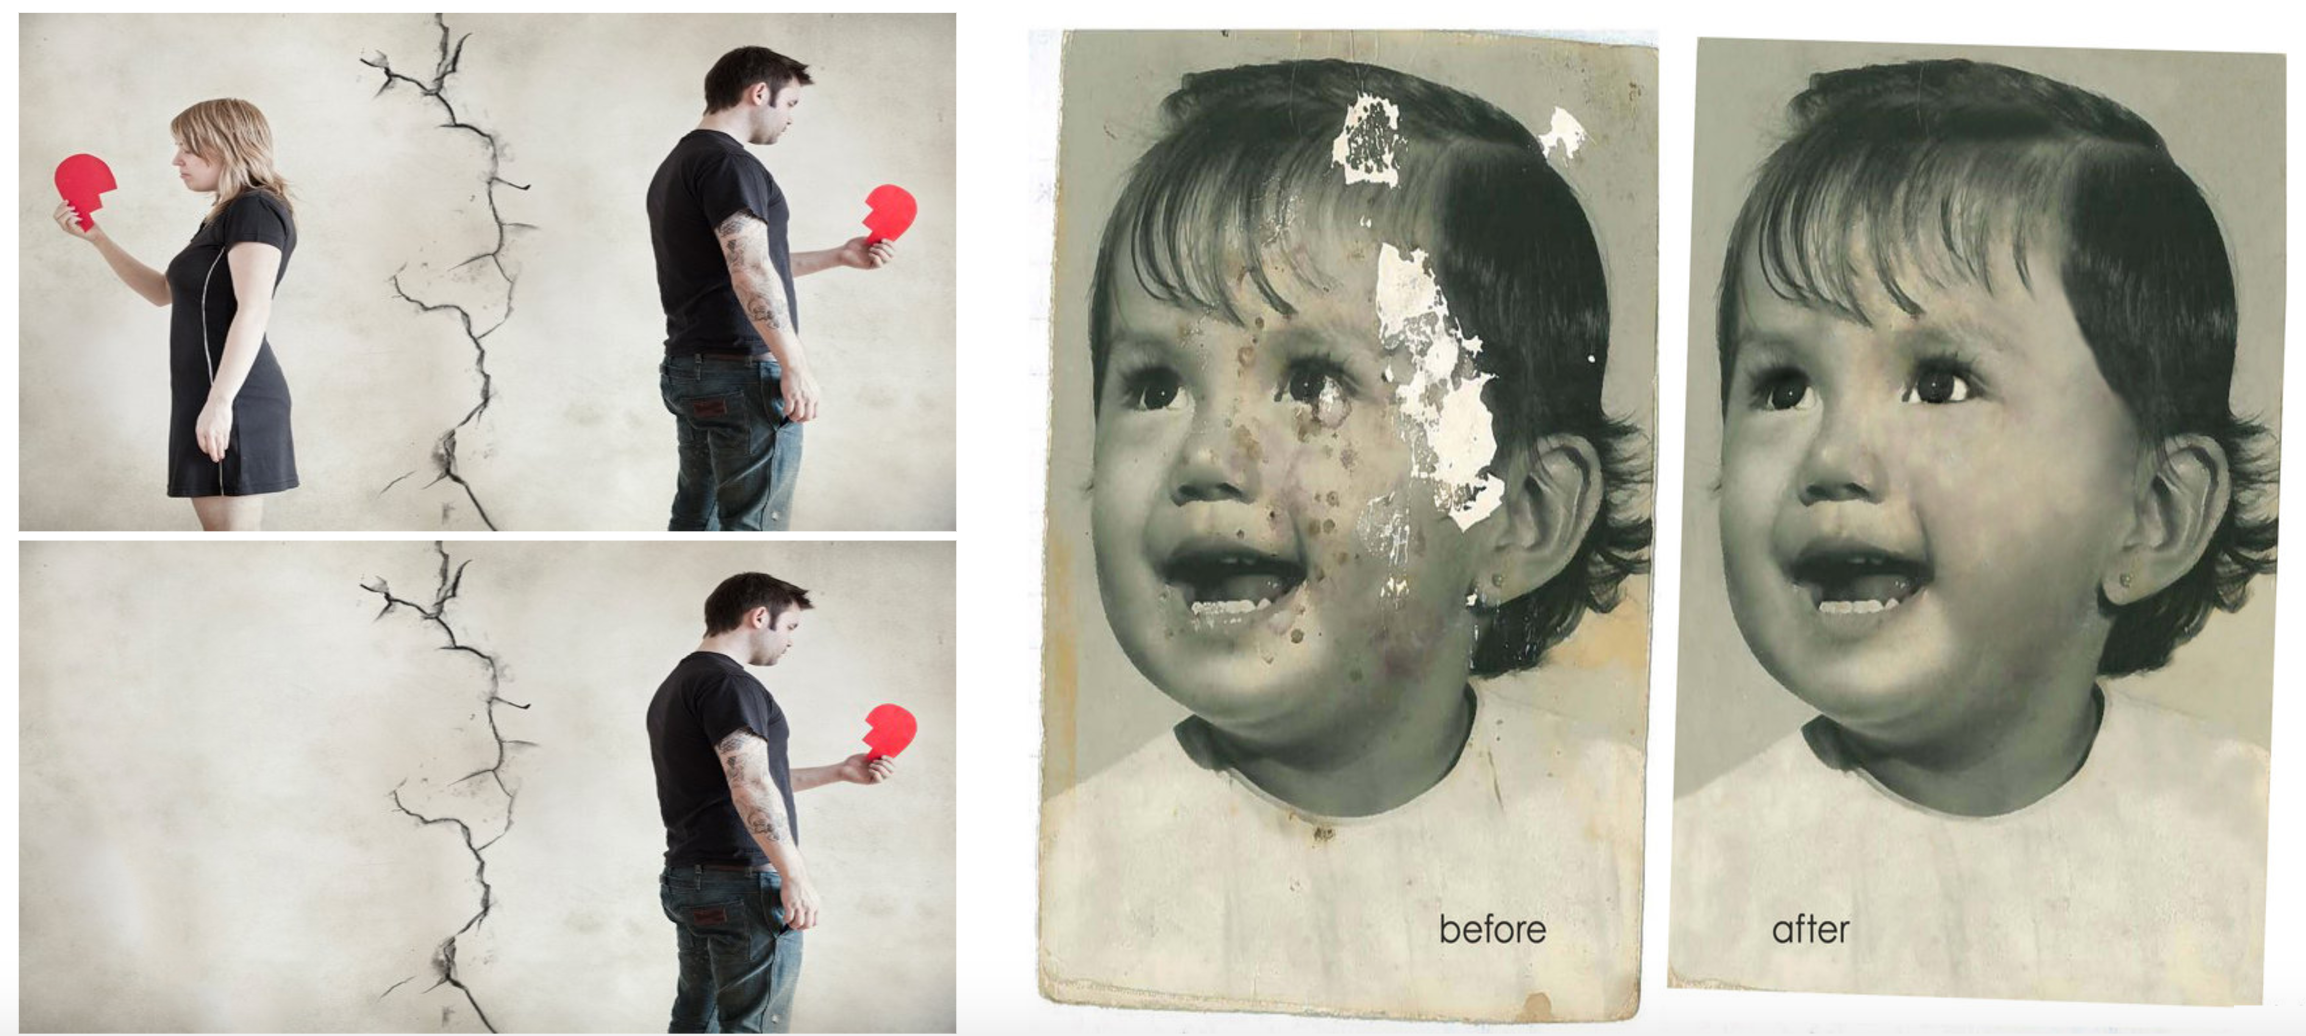
\includegraphics[width=1\columnwidth]{figures/problem.png}
\end{center}
\end{minipage}
Imaging you would like to edit a photo after breaking up, or restore an old picture from damages, we designed a MULTI-SCALE DEEP LEARNING algorithm to help you! Our approach
\begin{itemize}
\item proposed a joint optimization framework that can hallucinates missing image regions by modeling a global content constraint and local texture constraint with convolutional neural networks.
\item further introduced a multi-scale neural patch synthesis algorithm for high-resolution image inpainting based on the joint optimization framework.
\end{itemize}
\vspace{0.3em} % When there are two boxes, some whitespace may need to be added if the one on the right has more content
}


\headerbox{The Algorithm}{name=algorithm,column=0,span=1, 
 below=objectives}{
 \vspace{0.6cm}
\begin{minipage}[t]{1\linewidth}
\begin{center}
\begin{tabular}{rl}
\hline\noalign{\smallskip}
\multicolumn{2}{l}{\textbf{High-Resolution Hole Filling}}\\
\multicolumn{2}{l}{\textbf{with Multi-Scale Neural Patch Synthesis}}\\
\hline\noalign{\smallskip}
\multicolumn{2}{l}{\textbf{Input:} Image $x$, }\\ 
& the content network $f$, \\
& the texture network $t$,\\
& the number of scales $N$ \\
1: & Downsize $x$ to $128\times 128$. \\
2: & Compute the initial content reference $x^1$. \\ 
   & by giving $x$ as input to $f$.\\
3: & \textbf{for} $s \in [1, 2, \dots , N]$: \\
4. & Initialize $\tilde{x}=x^s$. \\
4: & Update $\tilde{x}$ that minimizes the joint loss:\\
   & $L=L_{content}+L_{texture}+L_{tv-smoothness}$. \\
5: & Compute $x^{s+1} $ by up-sampling $\tilde{x}$.\\  
7: & \textbf{end for}\\
8: & Return $\tilde{x}^N$.\\
\hline
\end{tabular}
\end{center}
\end{minipage}
\vspace{0.6cm}
}

%----------------------------------------------------------------------------------------
%	INTRODUCTION
%----------------------------------------------------------------------------------------

\headerbox{The Content Network}{name=content,column=1,span=1, row=0}{
\begin{minipage}{1\linewidth}
\begin{minipage}[t]{1\linewidth}
\begin{center}
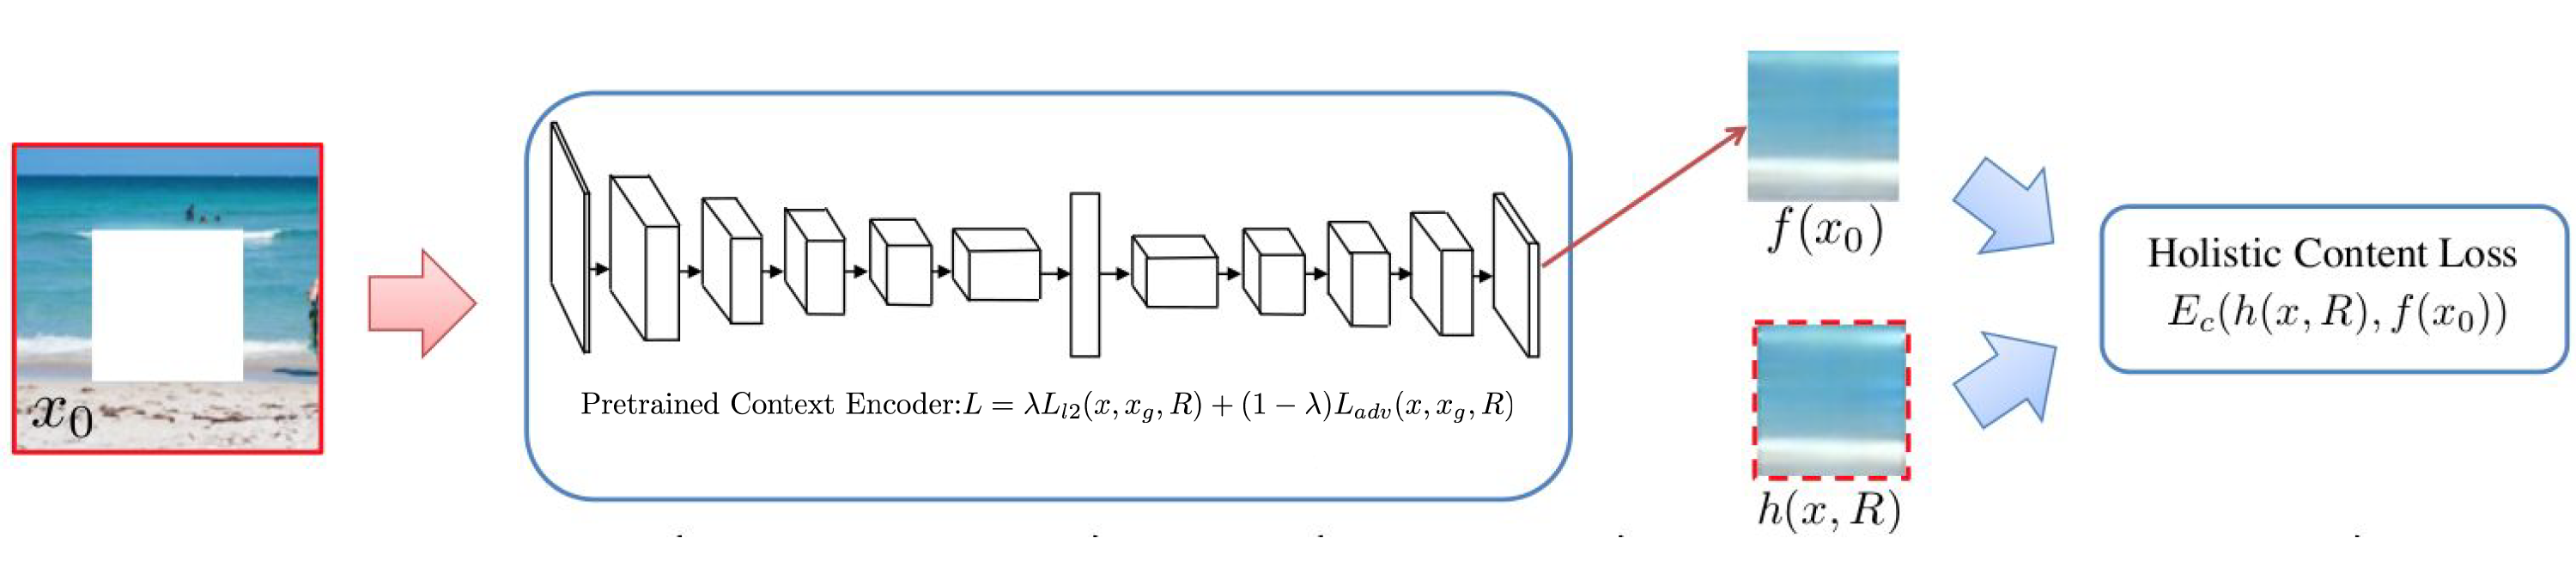
\includegraphics[width=1\columnwidth]{figures/content_network.png}
\end{center}
\end{minipage}
\begin{center}
\noindent\textbf{Context Encoder Predicts the Low-Res Content}
\end{center}
The content constraint: 
\begin{equation*}
E_c(h(x,R), h(x_i,R))  = \parallel h(x,R) - h(x_i,R) \parallel_2^2
\end{equation*}
\end{minipage}
}

\headerbox{The Texture Network}{name=texture,column=1,span=1, below=content}{
\begin{minipage}{1\linewidth}
\begin{minipage}[t]{1\linewidth}
\begin{center}
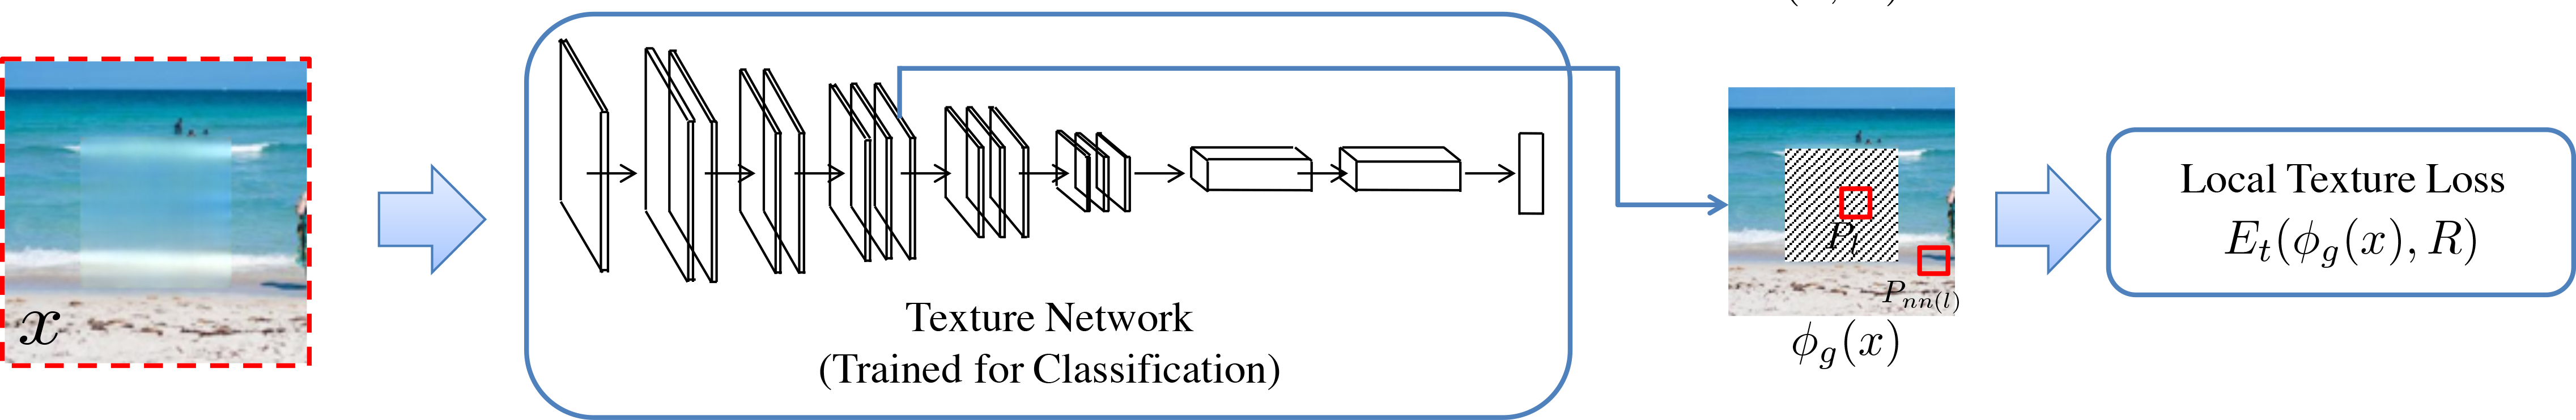
\includegraphics[width=1\columnwidth]{figures/texture_network.png}
\end{center}
\end{minipage}
\begin{center}
\noindent\textbf{Pre-trained VGG Optimizes the High-Res Texture}
\end{center}
The texture constraint:
\begin{multline}
E_t(\phi_t(x),R)  = \\ 
\frac{1}{|R^{\phi}|}\sum_{i\in R^{\phi}} \parallel h(\phi_t(x),P_i) - h(\phi_t(x),P_{nn(i)})  \parallel_2^2 \nonumber
\end{multline}
\end{minipage}
}

\headerbox{The Joint Loss Function}{name=loss,column=1,span=1,below=texture}{
At each iteration, we minimize:\\
\begin{minipage}{1\linewidth}
\begin{eqnarray*}
\tilde{x}_{i+1} = & \argmin_{x} E_c(h(x,R), h(x_i,R)) \nonumber \\ 
& +\alpha E_t(\phi_t(x),R^{\phi})  + \beta \Upsilon(x)
\label{eq:opt}
\end{eqnarray*}
\end{minipage}
}

\headerbox{Multi-scale Optimization}{name=multiscale,column=1,span=1,bottomaligned = algorithm, below=loss}{
We optimize at three scales: 128, 256 and 512:
\vspace{0.4cm}
\begin{minipage}[t]{1\linewidth}
\begin{center}
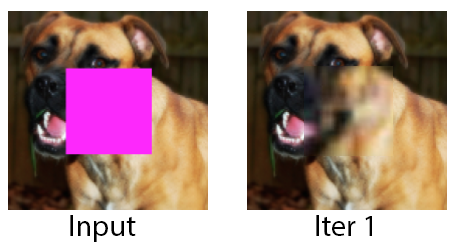
\includegraphics[width=0.5\columnwidth]{figures/multiscale_1.png}\\
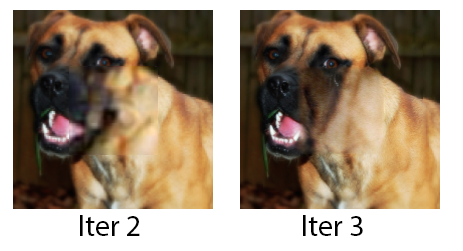
\includegraphics[width=0.5\columnwidth]{figures/multiscale_2.png}
\end{center}
\end{minipage}
}

\headerbox{\small Changing the Texture Weight $\alpha$}{name=weight,column=2,span=1, row=0}{ % This block's bottom aligns with the bottom of the conclusion block
The weight $\alpha$ measures the contribution of the texture constraint relative to the content constraint. It is a trade off between the sharpness of the texture and coherence of the structure: \\
\begin{minipage}{1\linewidth}
\begin{minipage}[t]{1\linewidth}
\setlength\tabcolsep{1.5pt}
\centering
\tiny
\begin{tabular}{cccc}
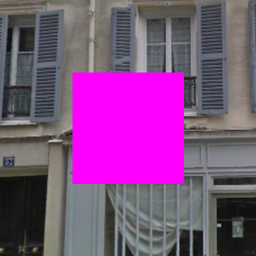
\includegraphics[width=.20\linewidth]{figures/pink_0046_r.png} &
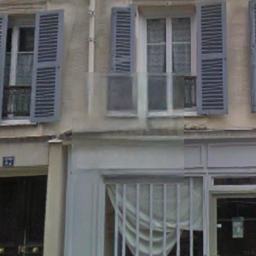
\includegraphics[width=.20\linewidth]{figures/res_3_100_1_r.png} &
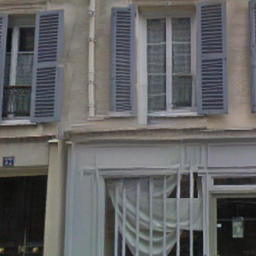
\includegraphics[width=.20\linewidth]{figures/res_3_100_2_r.png} &
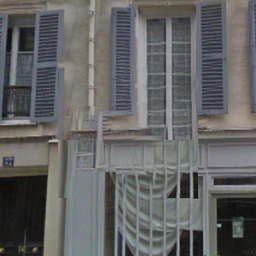
\includegraphics[width=.20\linewidth]{figures/res_3_100_3_r.png} \\
(a) Input image & (b) $\alpha=1e-6$ & (c) $\alpha=1e-5$ & (d) $\alpha=4e-5$\\ 
\end{tabular}
%\caption{The effect of texture weight $\alpha$. }\label{alpha}
\end{minipage}
\end{minipage}
}

\headerbox{\small Dropping the Content Constraint}{name=drop_content,column=2,span=1, below=weight }{ % This block's bottom aligns with the bottom of the conclusion block
Without using the content term to guide the optimization, the structure of the inpainting results is completely incorrect, although they are visually sharp:\\
\begin{minipage}{1\linewidth}
\begin{minipage}[t]{1\linewidth}
\setlength\tabcolsep{1.5pt}
\centering
\tiny
\begin{tabular}{cccc}
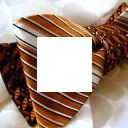
\includegraphics[width=.30\textwidth]{figures/ablation/pink_0065.jpg}&
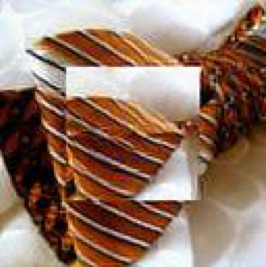
\includegraphics[width=.30\textwidth]{figures/ablation/no_content.jpg} &
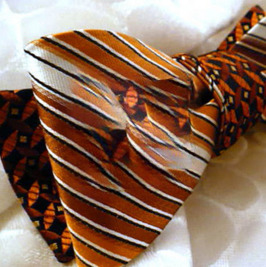
\includegraphics[width=.30\textwidth]{figures/ablation/result.jpg} \\
Input & Output without CN & Output with CN  \\ 
\end{tabular}
%\caption{The effect of texture weight $\alpha$. }\label{alpha}
\end{minipage}
\end{minipage}
}

\headerbox{\small Dropping the Adversarial Loss}{name=drop_adversarial,column=2,span=1, below=drop_content}{ 
When the initial prediction is blurry (using $\ell_2$ loss only), the final result becomes blurrier as well comparing with using the content network trained with both $\ell_2$ and adversarial loss.
\begin{minipage}{1\linewidth}
\centering
%\begin{minipage}[t]{1\linewidth}
\setlength\tabcolsep{1pt}
\tiny
\begin{tabular}{cccc}
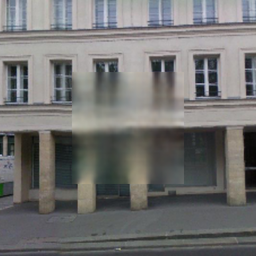
\includegraphics[width=.24\linewidth]{figures/fig2/fake_0049_l2_r.png} &
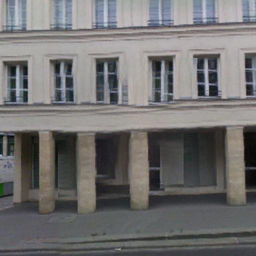
\includegraphics[width=.24\linewidth]{figures/fig2/res_3_100_r.png} & 
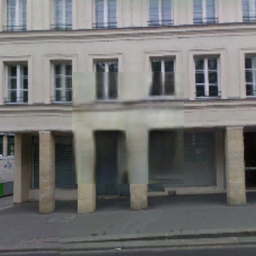
\includegraphics[width=.24\linewidth]{figures/fig2/fake_0023_adversarial_r.png} &
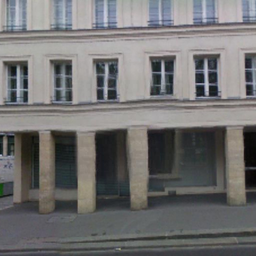
\includegraphics[width=.24\linewidth]{figures/fig2/no_bdry_0023_r.png} \\
(a) CN with $\ell_2$ loss & (b) (a)'s final output  & (c) CN with $\ell_2$ \& Adv loss & (d) (c)'s final output. \\ 
\end{tabular}
%\end{minipage}
\end{minipage}
}
\headerbox{\small Overall Comparison with Other Methods}{name=comparison,column=2,span=1, below=drop_adversarial}{
\begin{minipage}{1\linewidth}
\begin{center}
 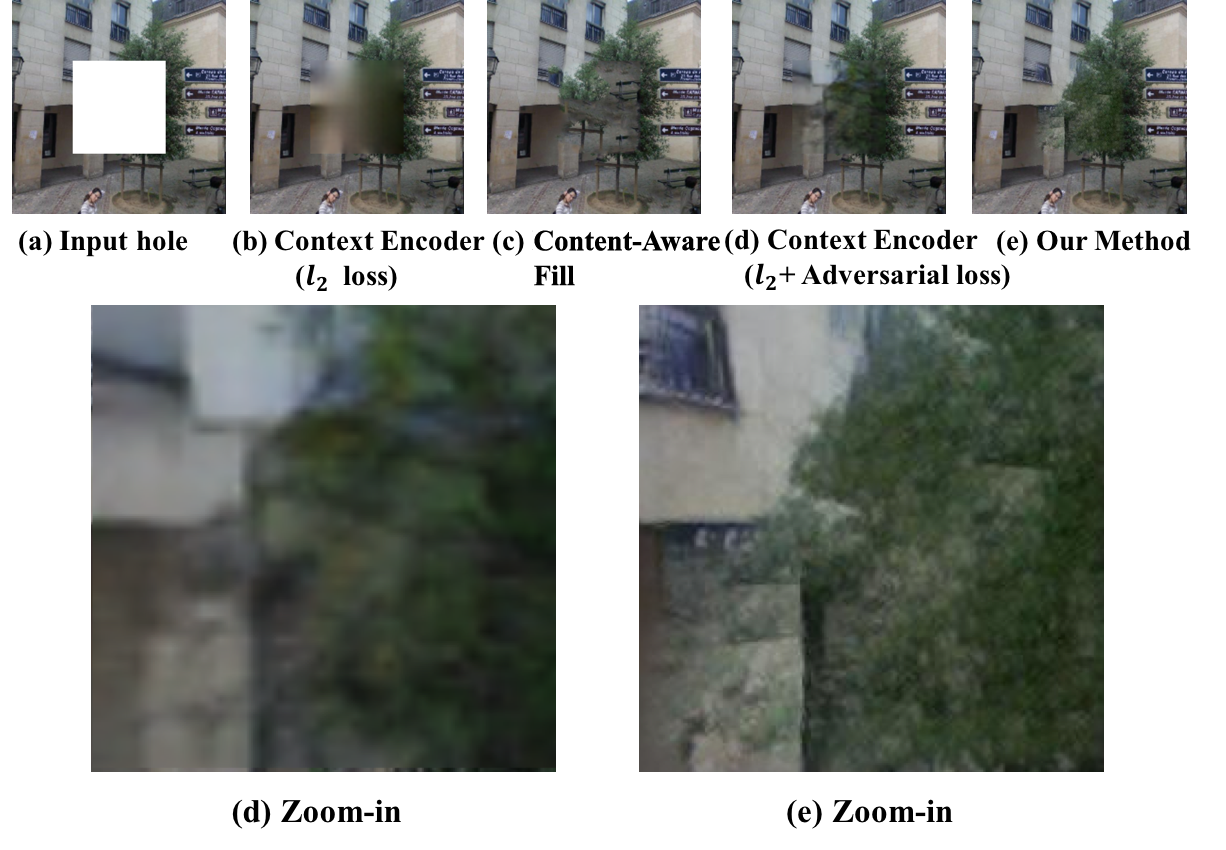
\includegraphics[width=0.85\linewidth]{figures/low_res/low_res2_3_3.png}
\end{center}
\end{minipage}
\vspace{-0.2cm}
}

\headerbox{\small We Love Cats and Dogs}{name=imagenet,column=3,span=1, row=0}{ 
And we have collected so many dogs and cats for you:\\
\begin{minipage}{1\linewidth}
\setlength\tabcolsep{1.5pt}
\centering
\tiny
\begin{tabular}{cccc}
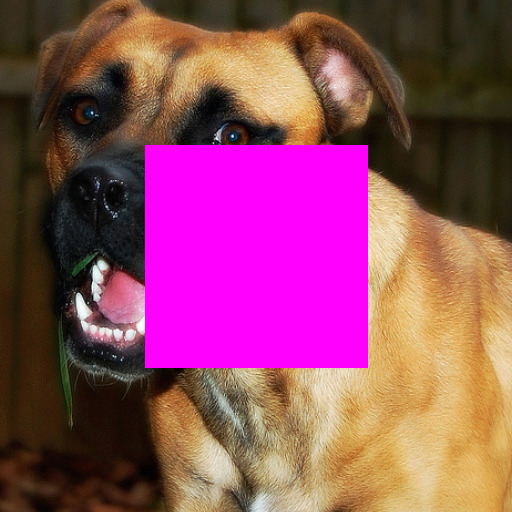
\includegraphics[width=.24\linewidth]{figures/pink_0076.jpg} &
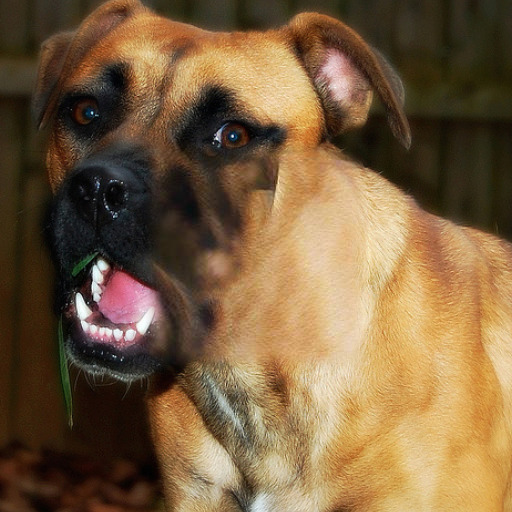
\includegraphics[width=.24\linewidth]{figures/no_bdry_0076.jpg} &
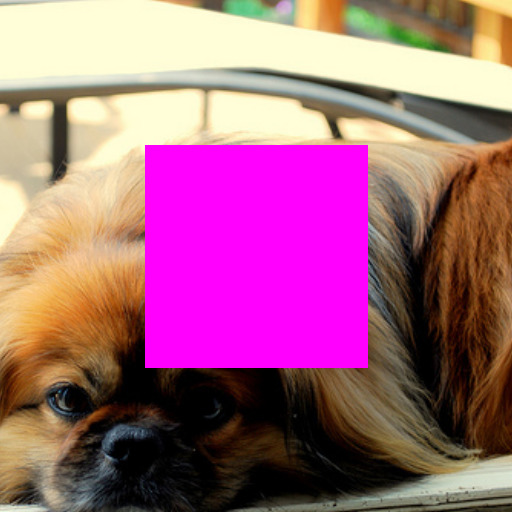
\includegraphics[width=.24\linewidth]{figures/pink_0081.jpg} &
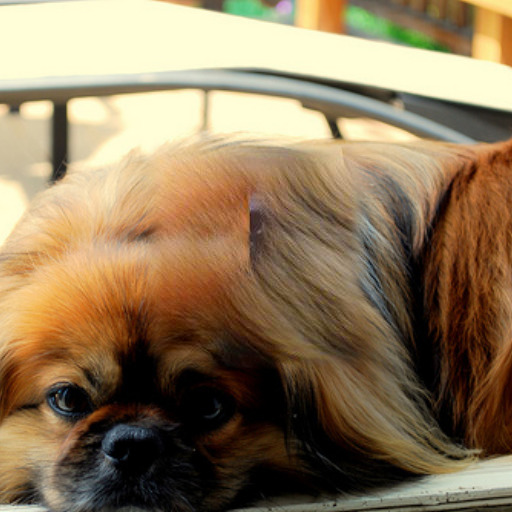
\includegraphics[width=.24\linewidth]{figures/no_bdry_0081.jpg} \\
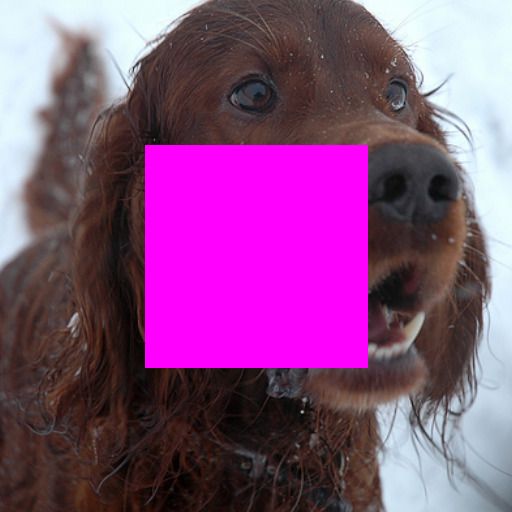
\includegraphics[width=.24\linewidth]{figures/pink_0082.jpg} &
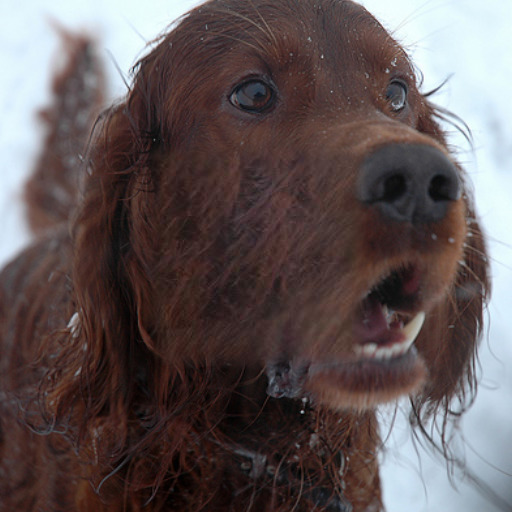
\includegraphics[width=.24\linewidth]{figures/no_bdry_0082.jpg} &
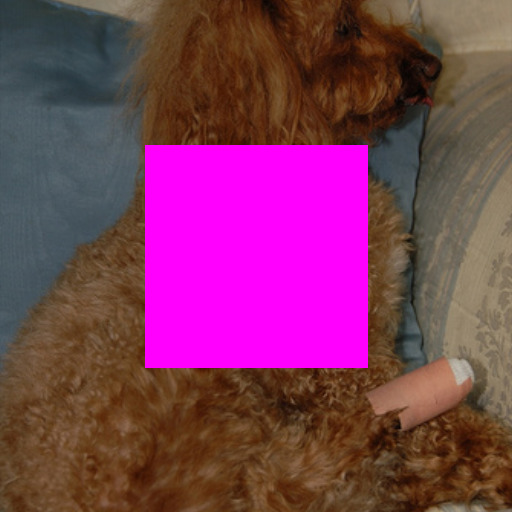
\includegraphics[width=.24\linewidth]{figures/pink_0154.jpg} &
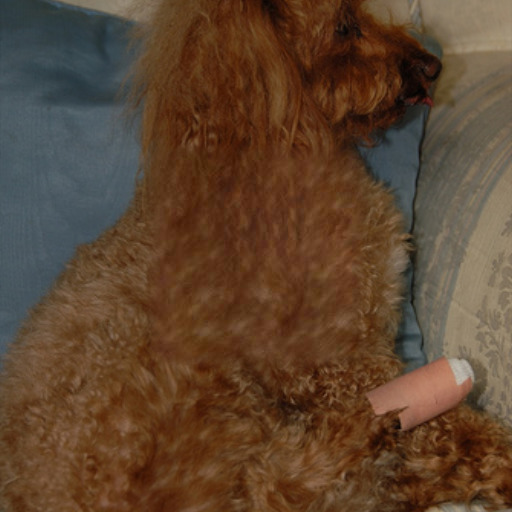
\includegraphics[width=.24\linewidth]{figures/no_bdry_0154.jpg} \\
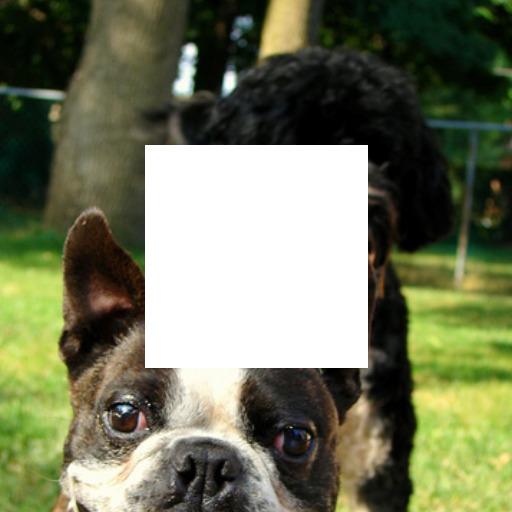
\includegraphics[width=.24\linewidth]{figures/pink_0071.jpg} &
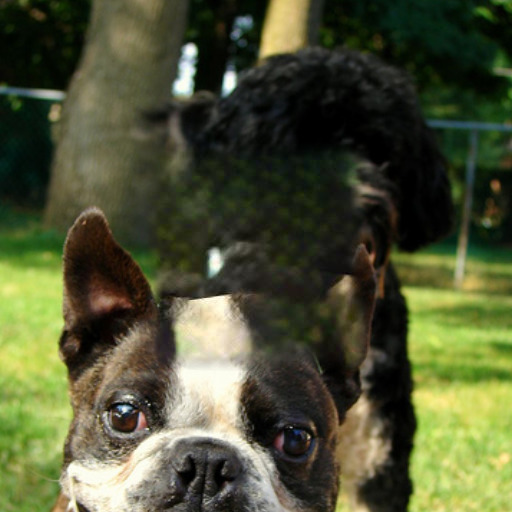
\includegraphics[width=.24\linewidth]{figures/no_bdry_0071.jpg} &
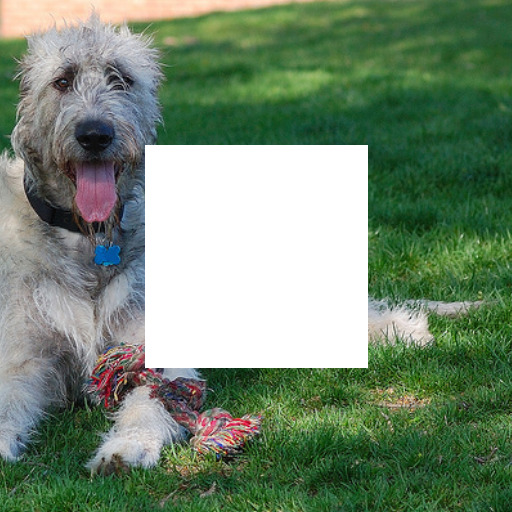
\includegraphics[width=.24\linewidth]{figures/pink_0097.jpg} &
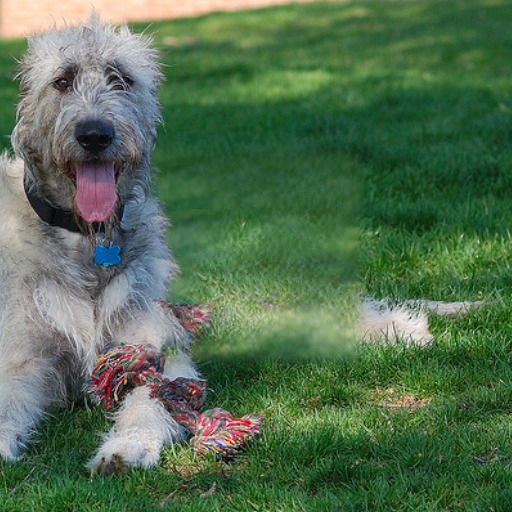
\includegraphics[width=.24\linewidth]{figures/no_bdry_0097.jpg} \\
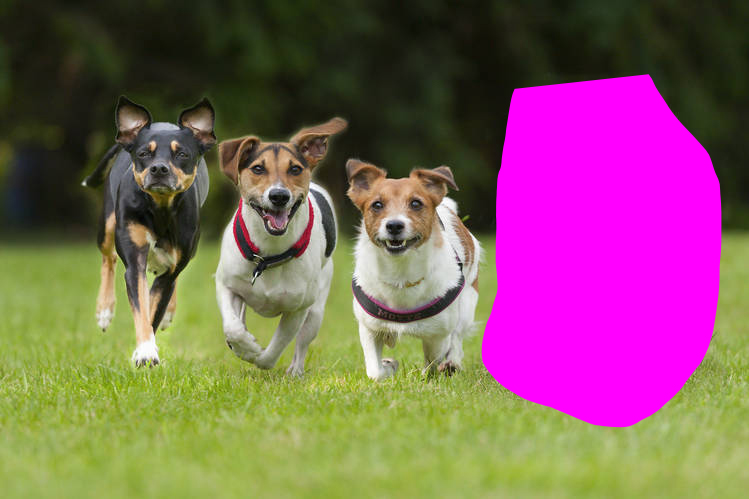
\includegraphics[width=.24\linewidth]{figures/dog_hole.jpg} &
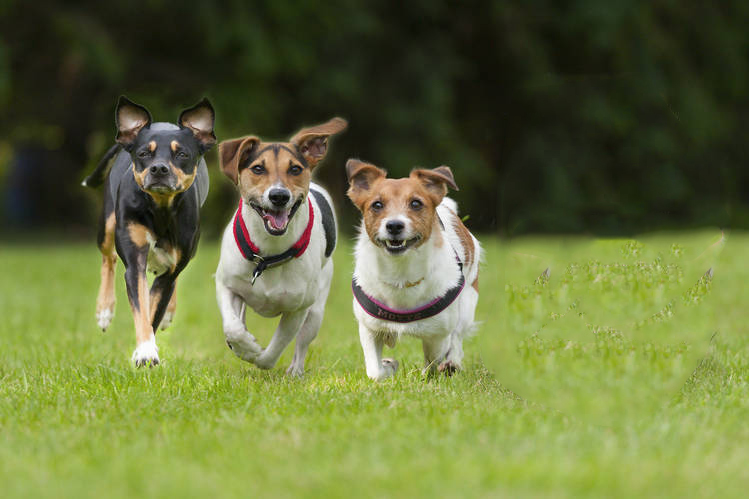
\includegraphics[width=.24\linewidth]{figures/res_3_100.jpg} &
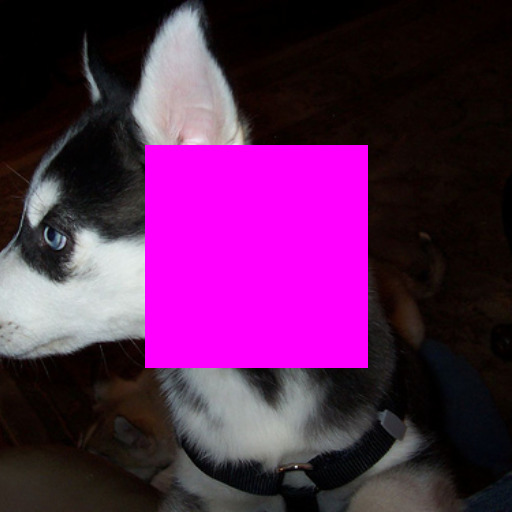
\includegraphics[width=.24\linewidth]{figures/pink_0342.jpg} &
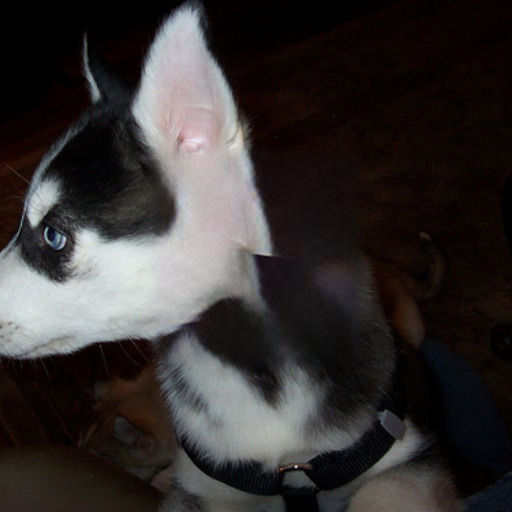
\includegraphics[width=.24\linewidth]{figures/no_bdry_0342.jpg} \\ 
\end{tabular}
%\caption{The effect of texture weight $\alpha$. }\label{alpha}
\end{minipage}
}

\headerbox{\small And What Inpaints Paris Like Paris?}{name=paris,column=3,span=1, below=imagenet}{ 
\begin{minipage}{1\linewidth}
\setlength\tabcolsep{1.5pt}
\centering
\tiny
\begin{tabular}{cccc}
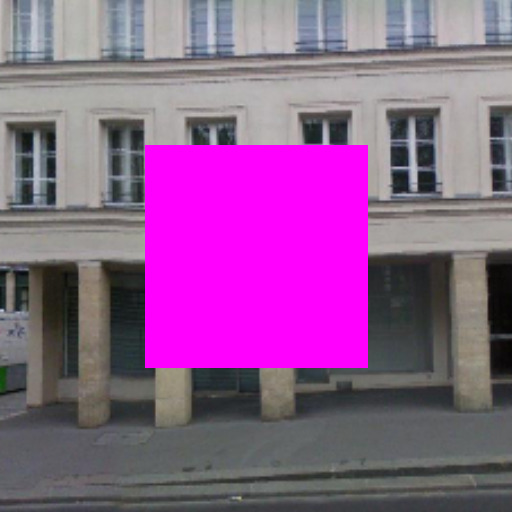
\includegraphics[width=.24\linewidth]{figures/paris/pink_0023.jpg} &
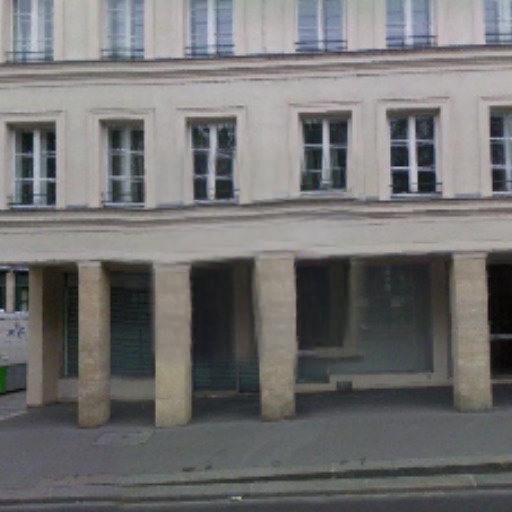
\includegraphics[width=.24\linewidth]{figures/paris/no_bdry_0023.jpg} &
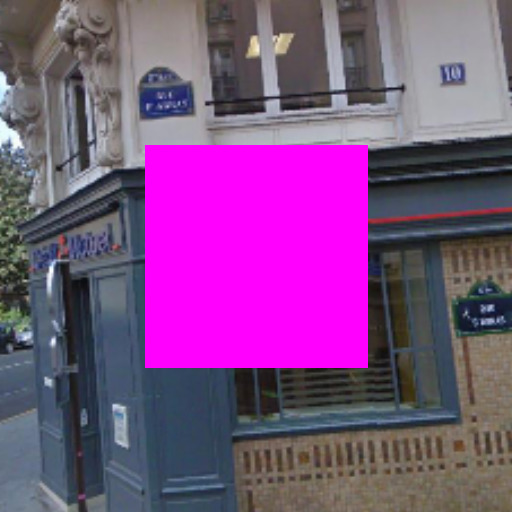
\includegraphics[width=.24\linewidth]{figures/paris/pink_0048.jpg} &
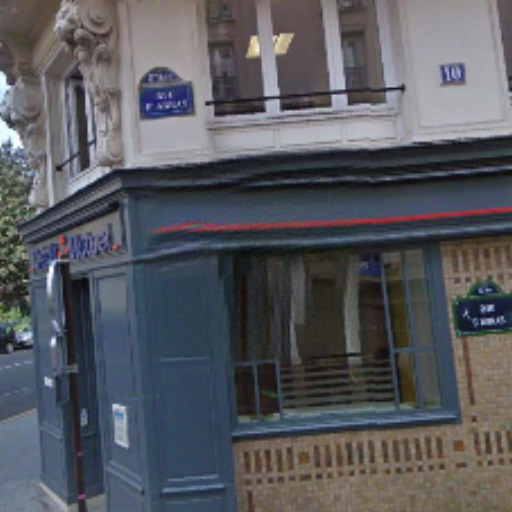
\includegraphics[width=.24\linewidth]{figures/paris/no_bdry_0048.jpg} \\
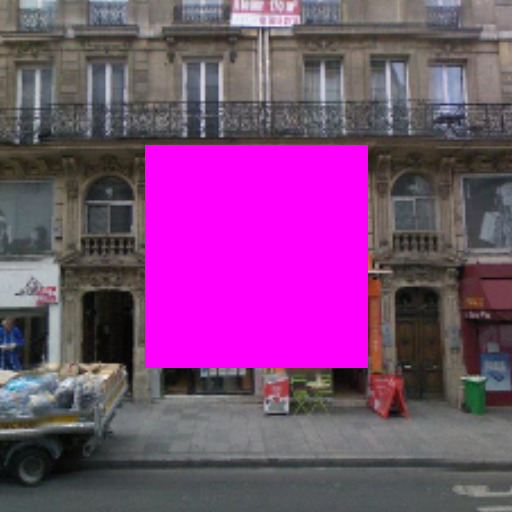
\includegraphics[width=.24\linewidth]{figures/paris/pink_0078.jpg} &
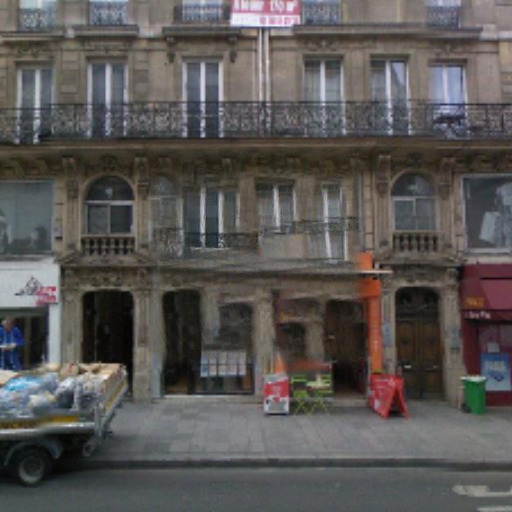
\includegraphics[width=.24\linewidth]{figures/paris/no_bdry_0078.jpg} &
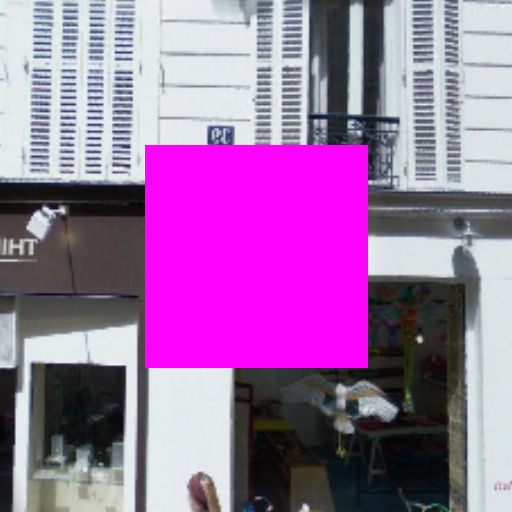
\includegraphics[width=.24\linewidth]{figures/paris/pink_0085.jpg} &
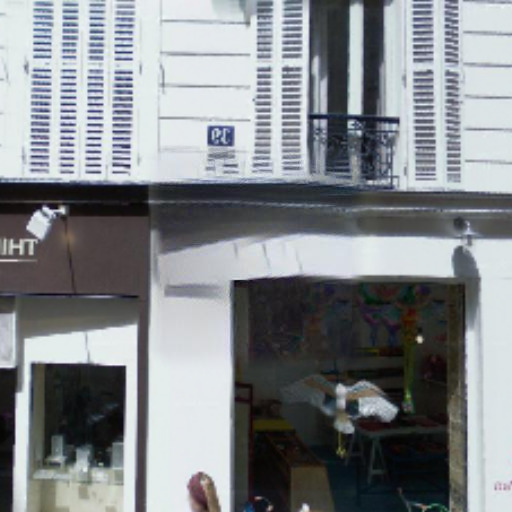
\includegraphics[width=.24\linewidth]{figures/paris/no_bdry_0085.jpg} \\
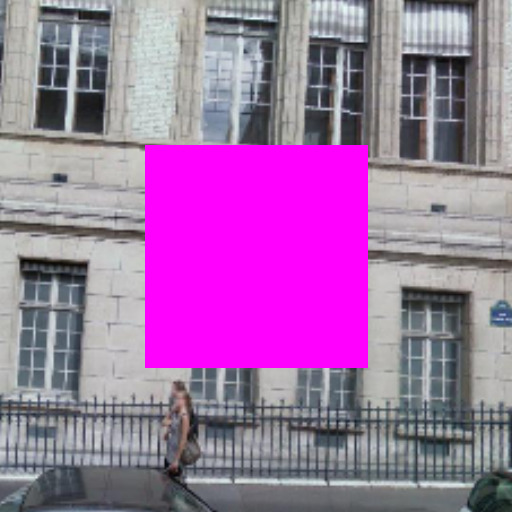
\includegraphics[width=.24\linewidth]{figures/paris/pink_0097.jpg} &
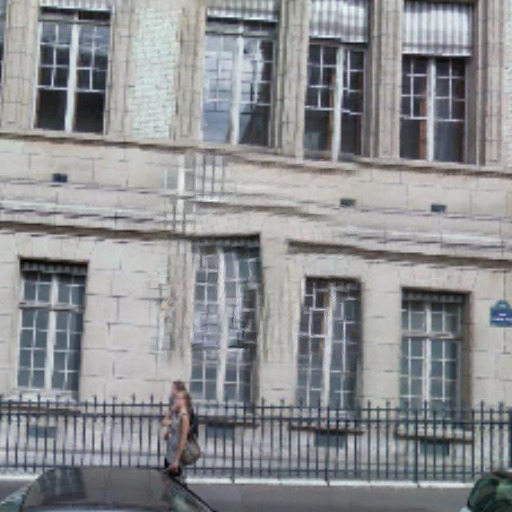
\includegraphics[width=.24\linewidth]{figures/paris/no_bdry_0097.jpg} &
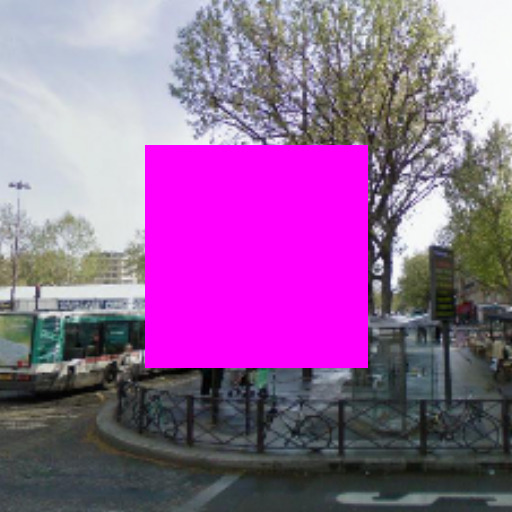
\includegraphics[width=.24\linewidth]{figures/paris/pink_0119.jpg} &
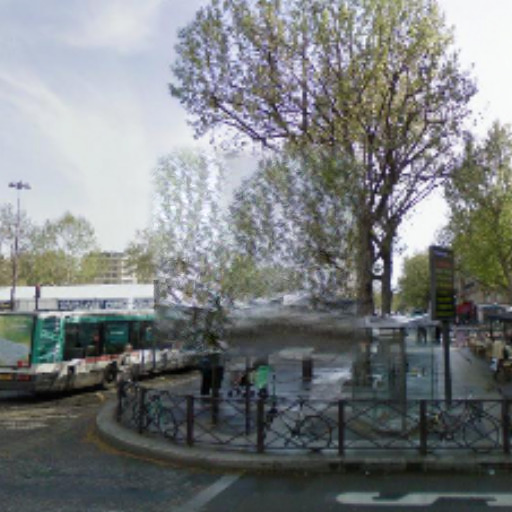
\includegraphics[width=.24\linewidth]{figures/paris/no_bdry_0119.jpg} \\
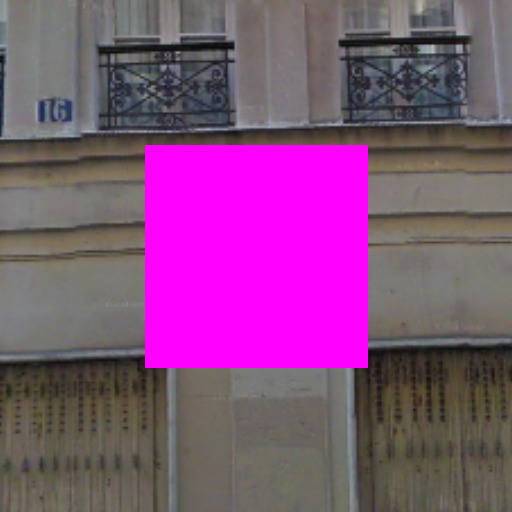
\includegraphics[width=.24\linewidth]{figures/paris/pink_0165.jpg} &
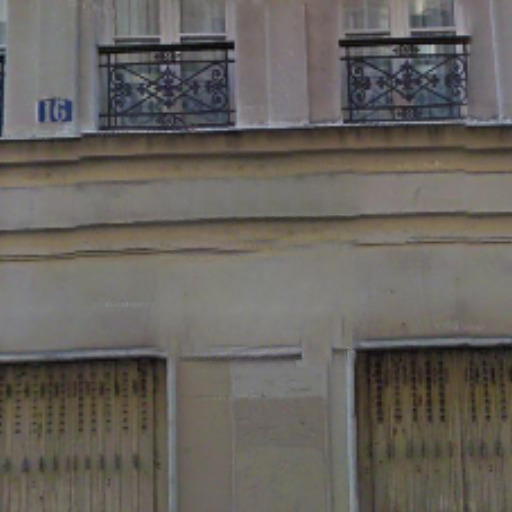
\includegraphics[width=.24\linewidth]{figures/paris/no_bdry_0165.jpg} &
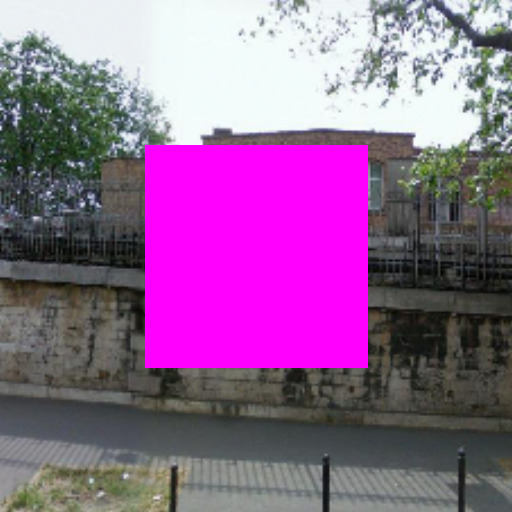
\includegraphics[width=.24\linewidth]{figures/paris/pink_0183.jpg} &
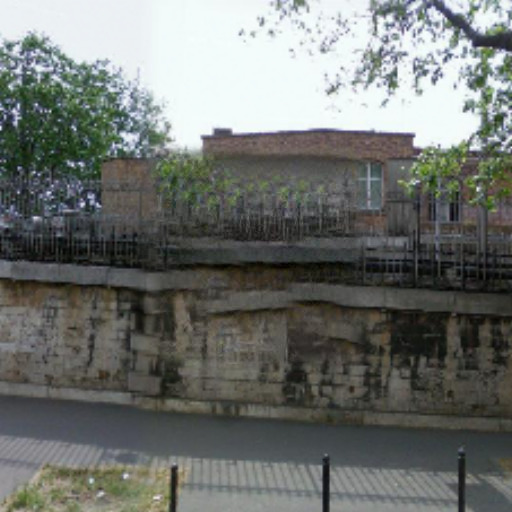
\includegraphics[width=.24\linewidth]{figures/paris/no_bdry_0183.jpg} \\

\end{tabular}
%\caption{The effect of texture weight $\alpha$. }\label{alpha}
\end{minipage}
}

\headerbox{\small For Paper, Results, Code and More}{name=qr,column=3,span=1, below=paris}{
\vspace{-0.1cm}
\begin{minipage}{1\linewidth}
\begin{center}
 \includegraphics[width=0.15\linewidth]{figures/qr_code.jpg}
\end{center}
\end{minipage}
\vspace{-0cm}
}
%----------------------------------------------------------------------------------------


\end{poster}

\end{document}